\section*{2}

Obtenga el cono contingente al conjunto
\begin{equation*}
    S := \{ (x, y) \in \R^2 : y \geq (x - 3)^2 + 3 \text{ and } y \leq -x + 8 \},
\end{equation*}
en el punto $(4, 4)$, y determine una base para este cono.

\noindent\rule{10cm}{0.4pt}

Sean $f(x):= (x - 3)^2 + 3$ y $g(x) := -x + 8$, 
derivando tenemos que
\begin{equation*}
    f'(x) = 2(x - 3), \qquad g'(x) = -1,
\end{equation*}
en particular $f'(4) = 2$ y $g'(4) = -1$.
por tanto el cono contingente a $S$ en el punto $(4, 4)$ viene dado por
\begin{equation*}
    T(S, (4, 4)) = \{ \lambda (-1, a) : \lambda \geq 0 \text{ and } a \in [-2, 1] \}.
\end{equation*}

\begin{figure}[h]
\centering
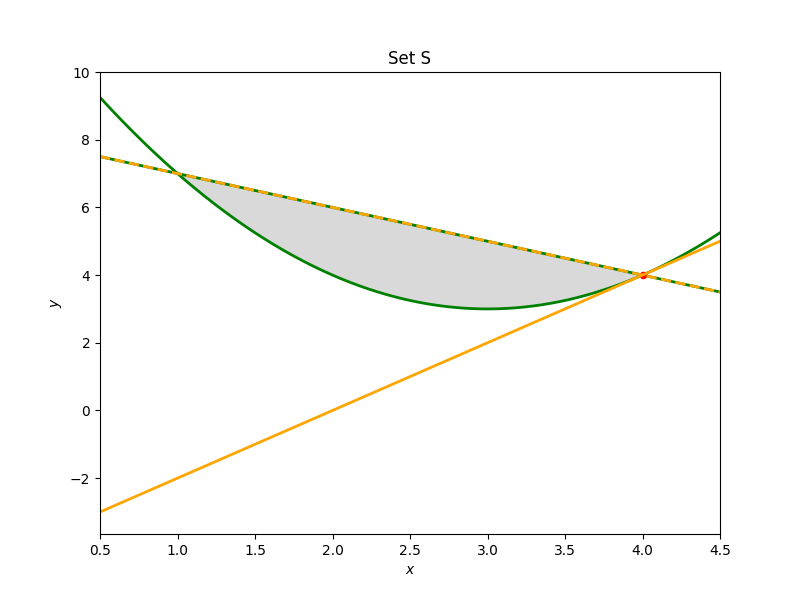
\includegraphics[scale=0.6]{pec3_ex2_setS.png}
\caption{
    Conjunto $S$ y los vectores tangentes en $(4,4)$.
}
\label{ex2_plot_set}
\end{figure}

Una base de $T(S, (4, 4))$ se puede obtener interescando la recta $(-1, y)$ para todo $y$ con el conjunto $T(S, (4,4))$,
de modo que
\begin{equation*}
    B = \{ (-1, y) : y \in [-2, 1] \},
\end{equation*}
es una base de $T(S, (4, 4))$.

\begin{figure}[h]
\centering
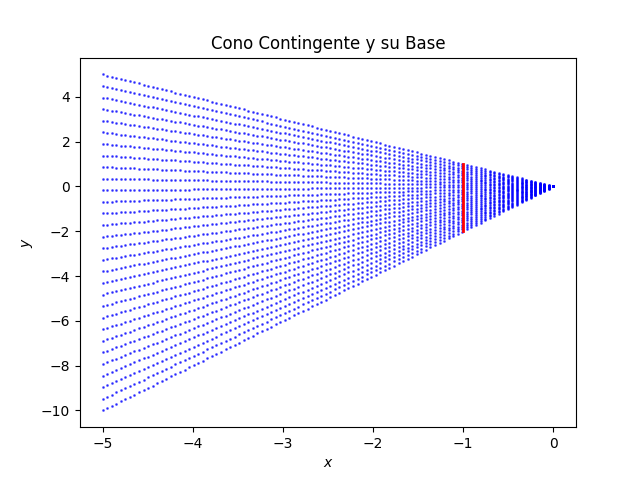
\includegraphics[scale=0.6]{pec3_ex2_TS.png}
\caption{
    Cono contingente y su base.
}
\label{ex2_plot_TS}
\end{figure}
